\documentclass{article}
\usepackage[utf8]{inputenc}
\usepackage[spanish]{babel}
\usepackage{listings}
\usepackage{graphicx}
\graphicspath{ {images/} }
\usepackage{cite}

\begin{document}

\begin{titlepage}
    \begin{center}
        \vspace*{1cm}
            
        \Huge
        \textbf{Ideación del proyecto final}
            
        \vspace{0.5cm}
        \LARGE
        Evil Dreams
            
        \vspace{1.5cm}
            
        \textbf{Mario Andres Leal Galvis\\
        Juan Camilo Mazo Castro}
            
        \vfill
            
        \vspace{0.8cm}
            
        \Large
        Despartamento de Ingeniería Electrónica y Telecomunicaciones\\
        Universidad de Antioquia\\
        Medellín\\
        Septiembre de 2021
            
    \end{center}
\end{titlepage}

\tableofcontents
\newpage
\section{Historia}
Tulio es un hombre que tenía una vida normal y una familia a la que amaba. Un día al salir del trabajó tuvo un accidente automovilístico y termina internado en una clínica en coma. Un día después de un largo tiempo despierta en aquella clínica y se ve envuelto en todo un infierno, debe salir de este lugar repleto de monstruos para encontrar a su familia y averiguar qué les sucedió. Al salir de la clínica se dirige rumbo hacia a su casa, tras pasar por muchos obstáculos y llegar al fin a su casa; se encuentra con un demonio mucho más poderoso que tiene a su familia como prisionera, Tulio lo debe derrotar para rescatarlos.
\newpage

\section{Descripción del juego} \label{contenido1} 
El juego es de tipo rpg con vista desde arriba.ambientado en un personaje que se despierta de un coma y se encuentra en un mundo con demonios que quieren acabar con su vida.Este contará con dos o tres enemigos y un boss final.Tambien, contará con 3 niveles y en cada nivel tendrá diferentes enemigos.\\

\begin{figure}[ht]
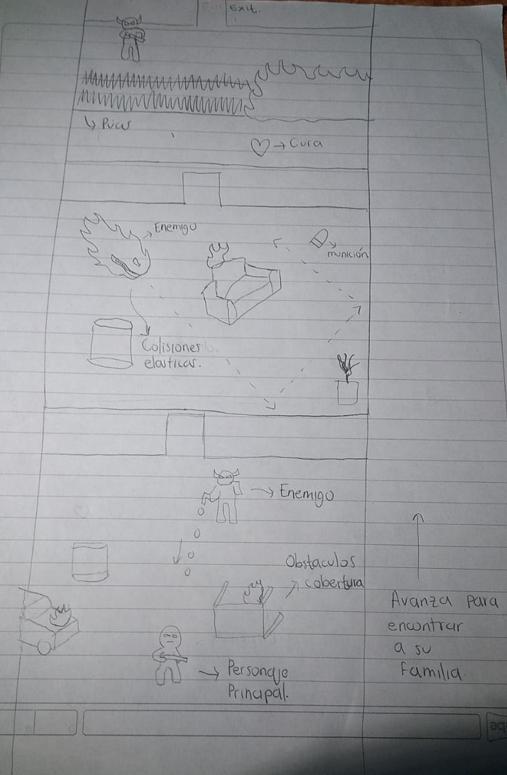
\includegraphics[width=7cm]{juego.png}
\centering
\caption{Idea del mapa}
\label{fig:juego}
\end{figure}

\subsection{Objetivo}
El personaje tendrá que superar  los diferentes niveles sobreviviendo para poder derrotar al jefe final para liberar su familia.

\subsection{Jugador}
El jugador podrá tener movimientos hacia arriba,abajo,derecha e izquierda, podrá disparar a cualquier dirección para eliminar enemigos y estamos evaluando la posibilidad de esquivar ataques.
Podrá recoger munición y vida. El jugador tendrá que cuidar su munición ya que contará con 15 balas, cada bala inflingirá 10 de daño. Si se queda sin munición no podrá disparar y deberá recoger más munición.El personaje contará con 100 de vida.

\subsection{Enemigos}

\begin{itemize}
\item{\textbf{Hechicero maldito:} }   Demonio que dispara balas de fuego, cada bola de fuego hace un daño de 20. El hechicero contará con una vida de 30.
\end{itemize} 
\begin{itemize}
    \item {\textbf{Rebotín:}} Demonio que rebota en las paredes e intenta embestir al personaje principal, cada embestida hace un daño de 10. 
\end{itemize}
\begin{itemize}
    \item {\textbf{Fuego:}} El fuego se encuentra en el entorno y si el jugador lo toca, recibe un daño de 12.
\end{itemize}
\begin{itemize}
    \item {\textbf{Pinchos:}} Los pinchos se encuentran también en el entorno, si el jugador los toca recibe un daño de 15.
\end{itemize}
\begin{itemize}
    \item {\textbf{Satanás:}} Jefe final que se encuentra en el último nivel. Tiene una vida de 150 y puede lanzar ondas de bolas de fuego. Con cada cierto porcentaje de vida su ataque cambia, se incinera e intenta embestir al jugador.
\end{itemize}

\end{document}
